
\documentclass[10pt,journal,compsoc]{IEEEtran}

\usepackage{graphicx}
\usepackage{amsmath}
\usepackage{algorithm}
\usepackage{algpseudocode}
% *** CITATION PACKAGES ***
%
\ifCLASSOPTIONcompsoc
  % The IEEE Computer Society needs nocompress option
  % requires cite.sty v4.0 or later (November 2003)
  \usepackage[nocompress]{cite}
\else
  % normal IEEE
  \usepackage{cite}
\fi


% *** GRAPHICS RELATED PACKAGES ***
%
\ifCLASSINFOpdf

\else

\fi






\newcommand\MYhyperrefoptions{bookmarks=true,bookmarksnumbered=true,
pdfpagemode={UseOutlines},plainpages=false,pdfpagelabels=true,
colorlinks=true,linkcolor={black},citecolor={black},urlcolor={black},
pdftitle={Branch partitioning for top-down enumeration},%<!CHANGE!
pdfsubject={},%<!CHANGE!
pdfauthor={Iya Arefyeva, Spoorthi Nijalingappal},%<!CHANGE!
pdfkeywords={join-order optimization, top-down enumeration}}%<^!CHANGE!


% correct bad hyphenation here
\hyphenation{op-tical net-works semi-conduc-tor}


\begin{document}

\title{Branch partitioning for top-down enumeration}
\author{Iya Arefyeva,  Spoorthi Nijalingappa}% <-this % stops a space




% The paper headers
\markboth{}%
{{Iya Arefyeva, Spoorthi Nijalingappa}: (title)}
\IEEEtitleabstractindextext{%
\begin{abstract}
The abstract goes here.
\end{abstract}

% Note that keywords are not normally used for peerreview papers.
\begin{IEEEkeywords}
join-order optimization, top-down enumeration
\end{IEEEkeywords}}


% make the title area
\maketitle


\IEEEdisplaynontitleabstractindextext

\IEEEpeerreviewmaketitle


\ifCLASSOPTIONcompsoc
\IEEEraisesectionheading{\section{Introduction}\label{sec:introduction}}
\else
\section{Introduction}
\label{sec:introduction}
\fi

Introduction goes here

\section{Related works}
Overview of related methods goes here.

\section{Background}
\subsection{Basics}
\indent A query can be represented as a graph $G = (V, E)$, where vertices $V$ is the set of relations and edges $E$ are join predicates. For example, a vertex between two relations $R_1$ and $R_2$ exists if there is a join predicate that involves attributes of both $R_1$ and $R_2$. \\
\indent A \textit{join tree} is a binary tree where leaves represent relations and inner nodes represent sets of joined relations. A join tree defines an execution order of join operations. \\
\indent A graph $G = (V, E)$ is \textit{connected}, when there is a path between each pair of its vertices. \\
\indent The neighborhood of a vertex $v$ is defined as: $$N(v) = \{ w  |  w \in V \wedge (v, w) \in E\}$$
\indent Thus, the neighborhood of a set $S \subseteq E$ can be defined as:  $$N(v) = \{ w  |  v \in V \wedge w \in (V \setminus S) \wedge (v, w) \in E\}$$
\indent Two connected subgraphs $(S_1, S_2) \in G$ are called a connected subgraph and its complement pair (\textit{ccp}) if: \\
$S_1 \cap S_2 = \emptyset$ and $\exists (v_1, v_2) \in E$ such that $v_1 \in S_1 \wedge v_2 \in S_2$.

\subsection{Top-down enumeration}
\indent Top-down approaches use \textit{memorization} - a technique where previously computed results are cached and returned when the same computation is needed again. The generic top-down join enumeration \cite{FenderMCB} shown in Algorithm 1 stores the best join tree for a subgraph $S$ in $BestTree[S]$.\\
\indent In the beginning each vertex is assigned to BestTree for this vertex (line 3). Then TDPlanGenSub is called for the whole query graph $G$ (line 5). At every recursion step the algorithm finds all possible join trees for existing subtrees and keeps the cheapest one. \\
\indent TDPlanGenSub (Algorithm 2) recursively splits the subgraph $S$ and finds the best join tree for each partition. If the best tree for this partition already exists, the function simply returns it and uses in the parent invocation. \\
\indent BuildTree (Algorithm 3) is used to merge two join trees and assign the result to BestTree for the partition $S$ in case the cost for the created tree is lower than the cost for the tree previously saved in BestTree.

\begin{algorithm}
\caption{Pseudocode for TDPlanGen, taken from \cite{FenderMCB}}
\textbf{Input:} connected query graph $G = (V, E)$ \\
\textbf{Output:} an optimal join tree for $G$
\begin{algorithmic}[1]
\Procedure{TDPlanGen}{$G$}
\For {$i \leftarrow 1$ to $n$}
\State {$BestTree[v_i] \leftarrow v_i$}
\EndFor
\State {\textbf{return} $TDPlanGenSub(G)$}
\EndProcedure
\end{algorithmic}
\end{algorithm}

\begin{algorithm}
\caption{Pseudocode for TDPlanGenSub, taken from \cite{FenderMCB}}
\textbf{Input:} connected sub graph $S \subseteq G$ \\
\textbf{Output:} an optimal join tree for $S$
\begin{algorithmic}[1]
\Procedure{TDPlanGenSub}{$S$}
\If{$BestTree[S] = NULL$}
\ForAll {$ (S_1, S_2) \in Partition(S)$}
\State {$BuidTree(S, TDPlanGenSub(S_1), $ \phantom a \phantom . \phantom . \phantom . $TDPlanGenSub(S_2))$}
\EndFor
\EndIf
\State {\textbf{return} $BestTree[S]$}
\EndProcedure
\end{algorithmic}
\end{algorithm}

\begin{algorithm}
\caption{Pseudocode for BuildTree, taken from \cite{FenderMCB}}
\textbf{Input:} subgraph $S$, two sub join trees $Tree1, Tree2$ 
\begin{algorithmic}[1]
\Procedure{BuildTree}{$S, Tree1, Tree2$}
\State {$CurrentTree \leftarrow MergeTrees(Tree1, Tree2)$}
\If{$BestTree[S] = NULL  $ $\|$ $  cost(BestTee[S]) > cost(CurrentTree)$}
\State {$BestTree[S] \leftarrow CurrentTree$}
\EndIf
\State {$CurrentTree \leftarrow MergeTrees(Tree2, Tree1)$}
\If{$cost(BestTee[S]) > cost(CurrentTree)$}
\State {$BestTree[S] \leftarrow CurrentTree$}
\EndIf
\EndProcedure
\end{algorithmic}
\end{algorithm}


\subsection{Branch partitioning algorithm}
\subsubsection{Description}
\indent In order to find the best join tree for a query subgraph $S$ the algorithm should consider all possible pairs of connected subgraphs $(S_1, S_2)$ such that $S = S_1 \cup S_2$ and $S_1 \cap S_2 = \emptyset$. Thus, the task of a partitioning algorithm is to output a set of such pairs. \newline
\indent The branch partitioning algorithm (MinCutBranch) recursively enlarges a set $C$ by members of its neighborhood, starting with a single vertex $t \in S$. If $S \setminus C$ is connected as well, the algorithm emits the pair $(C, S \setminus C)$. Several additional sets are used to help achieving this:
\begin{itemize} 
\item One-element set $L$ that contains the last vertex $v$ added to $C$.
\item The result sets $R$ and $R_{tmp}$ of the current and the child invocation respectively.
\item The set $X$ of vertices that have already been used to enlarge $C$.
\item The set $N_L$ that contains all neighbors of $L$ that are not in $X$ and not in $C$.
\item The set $N_B$ that holds all neighbors of $C$ that are not neighbors of $L$ and additionally are not in $X$.
\item The set $N_X$ with neighbors of $L$ that are also elements of $X$, but are not in $C$.
\end{itemize}

\indent The MinCutBranch methods (Algorithm 5) considers three cases. The first case (line 8) is true when the intersection of set $N_B \cup N_L$ with the result set $R_{tmp}$ is not empty. It doesn't emit any partitions since they are already emitted in child invocations. \\
\indent The second case (line 15) is considered when the condition of the first case is not valid and the set $N_L$ is not empty. When MinCutBranch is just started, this case is always the first case to consider because $R_{tmp}$ is still empty. \\
\indent Else the third case (line 19) processes an element $v \in N_X$ and finds all neighbors of $C \cup \{v\}$ using the method Reachable (Algorithm 6). It returns the maximally enlarged and connected set adjacent to $L$, elements of which are not in $C$. The method starts with finding neighbors of $L$, then it iteratively finds neighbors of its neighbors etc. until there are no neighbors left. \\
\indent In the lines 24-32 the algorithms checks whether $R_{tmp}$ has already been submitted to avoid duplicates. If not, MinCutBranch emits the pair $(S \setminus R_{tmp}, R_{tmp})$. In the line 14 $X'$ is reset to $X$ so that later, while performing this check, the method doesn't falsely assume that the pair is a duplicate.\\

\begin{algorithm}
\caption{Pseudocode for Partition, taken from \cite{FenderMCB}}
\textbf{Input:} a connected set $S$
\begin{algorithmic}[1]
\Procedure{Partition}{$S$}
\State {$t \leftarrow$ arbitrary vertex of $S$}
\State {MinCutBranch($S, \{t\}, \emptyset, \{t\}$)}
\EndProcedure
\end{algorithmic}
\end{algorithm}

\begin{algorithm}
\caption{Pseudocode for MinCutBranch, taken from \cite{FenderMCB}}
\textbf{Input:} connected sets $S, C$ with $C, X \subset S, |L| = 1$ \\
\textbf{Output:} the result set $R \cup L$
\begin{algorithmic}[1]
\Procedure{MinCutBranch}{$S, C, X, L$}
\State $R \leftarrow \emptyset$
\State $R_{tmp} \leftarrow \emptyset$
\State $N_L \leftarrow ((N(L) \cap S) \setminus C) \setminus X$
\State $N_X \leftarrow ((N(L) \cap S) \setminus C) \cap X$
\State $N_B \leftarrow (((N(C) \cap S) \setminus C) \setminus N_L) \setminus X$
\While {$N_B \neq \emptyset \wedge N_X \neq \emptyset \vee N_B \cap R_{tmp} \neq \emptyset$}
\If {$(N_B \cup N_L) \cap R_{tmp} \neq \emptyset$} \Comment{Case 1}
	\State $v \leftarrow$ an element of $((N_B \cup N_L) \cap R_{tmp})$
	\State {MinCutBranch($S, C \cup \{v\}, X', \{v\}$)}
	\State $N_L \leftarrow N_L \setminus \{v\}$
	\State $N_B \leftarrow N_B \setminus \{v\}$
\Else
	\State $X' \leftarrow X$
	\If {$N_L \neq \emptyset$}  \Comment{Case 2}
		\State $v \leftarrow$ an element of $N_L$
		\State {$R_{tmp}= $MinCutBranch($S, C\cup\{v\}, X', \{v\}$)}
		\State $N_L \leftarrow N_L \setminus \{v\}$
	\Else  \Comment{Case 3}
		\State $v \leftarrow$ an element of $N_X$
		\State {$R_{tmp} =$ Reachable($S, C \cup \{v\}, \{v\}$)}
	\EndIf
	\State {$N_X = N_X \setminus R_{tmp}$}
	\If {$R_{tmp} \cap X \neq  \emptyset$}
		\State $N_X \leftarrow N_X \cup (N_L \setminus R_{tmp})$
		\State $N_L \leftarrow N_L \cap R_{tmp}$
		\State $N_B \leftarrow N_B \cap R_{tmp}$
	\EndIf
	\If {$(S \setminus R_{tmp}) \cap X \neq \emptyset$}
		\State $N_L \leftarrow N_L \cap R_{tmp}$
		\State $N_B \leftarrow N_B \cap R_{tmp}$
	\Else
		\State {emit ($S \setminus R_{tmp}, R_{tmp}$)}
	\EndIf
	\State $R \leftarrow R \cup R_{tmp}$
\EndIf
\State $X' \leftarrow X' \cup \{v\}$
\EndWhile
\State {\textbf{return} $R \cup L$}
\EndProcedure
\end{algorithmic}
\end{algorithm}

\begin{algorithm}
\caption{Pseudocode for Reachable, taken from \cite{FenderMCB}}
\textbf{Input:} connected sets $S, C \subseteq S, L \subseteq C, |L| = 1$ \\
\textbf{Output:} connected set $R$ adjacent to $C$
\begin{algorithmic}[1]
\Procedure{Reachable}{$S, C, L$}
\State $R \leftarrow L$
\State $N \leftarrow (N(L) \cap S) \setminus C$
\While {$N \neq \emptyset$}
\State $R \leftarrow R \cup N$
\State $N \leftarrow ((N(N) \cap S) \ C)$
\EndWhile
\State {\textbf{return} $R$}
\EndProcedure
\end{algorithmic}
\end{algorithm}

\subsubsection{Example}

The table on Figure 2 illustrates the execution steps of MinCutBranch for the cycle query graph (Figure 1). It shows depth of recursion, elements of sets $C$, $L$, $N_L$, $N_B$, $N_X$ and $X$ and the corresponding cases. The depth of recursion reaches the second level only once and immediately returns to the parent invocation, since the state of sets doesn't satisfy either of conditions of the cases.

\begin{figure}[h]
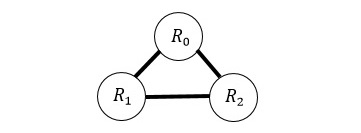
\includegraphics[width=0.5\textwidth]{graph.jpg}
\caption{Cycle query graph with three vertices}
\end{figure}

\begin{figure}[h]
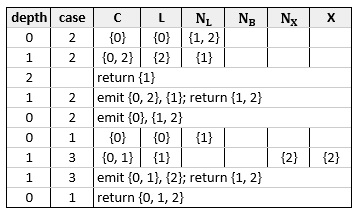
\includegraphics[width=0.5\textwidth]{table.jpg}
\caption{Example of execution of MinCutBranch}
\end{figure}

\section{Evaluation}
Evaluation goes here.

\section{Conclusion}
The conclusion goes here.



% use section* for acknowledgment
\ifCLASSOPTIONcompsoc
  % The Computer Society usually uses the plural form
  \section*{Acknowledgments}
\else
  % regular IEEE prefers the singular form
  \section*{Acknowledgment}
\fi


The authors would like to thank...

\ifCLASSOPTIONcaptionsoff
  \newpage
\fi


\begin{thebibliography}{1}

\bibitem{FenderMCB}
Fender, P. and Moerkotte, G., 2011, April. A new, highly efficient, and easy to implement top-down join enumeration algorithm. In 2011 IEEE 27th International Conference on Data Engineering (pp. 864-875). IEEE.

\end{thebibliography}



\end{document}


